%% Main results: mechanism isolation, cross-setting comparison, cost (Tables 4-6).
%% Included by sigconf.tex. Do not add a preamble here.

\section{Results}
\label{sec:results}

\begin{figure}[t]
\centering
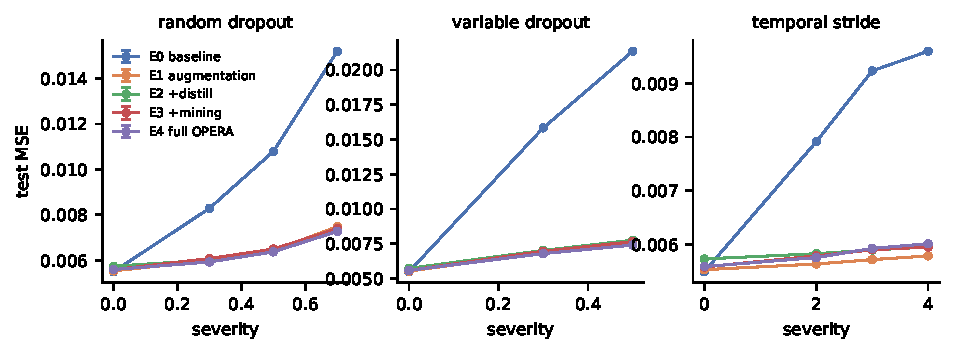
\includegraphics[width=\linewidth]{figures/fig3_robustness_curve.pdf}
\caption{Error against observation-process severity on PhysioNet\prelim, for three process families. Severity
$0$ is the dataset's own observation process. Without any mechanism (blue) error grows steeply in every family;
every OPERA configuration stays close to its clean error, including for stride subsampling, a family absent
from the training pool.}
\label{fig:curve}
\end{figure}

\paragraph{Exposure to diverse observation processes accounts for most of the attainable robustness.}
Table~\ref{tab:components} and Figure~\ref{fig:curve} isolate the mechanisms on PhysioNet. Augmentation alone
reduces $\Delta_{\mathrm{shift}}$ from $+107\%$ to $+14\%$ and $\Delta_{\mathrm{unseen}}$ from $+130\%$ to $+18\%$ while
leaving clean error unchanged ($0.00553$ vs.\ $0.00549$), and it improves all sixteen conditions. It transfers to
process families absent from training: stride subsampling, never trained on in any form, falls from $0.00923$ to
$0.00572$. On Activity the same mechanism, combined with the others, reduces mean shifted error from $0.04983$ to
$0.00358$, a factor of fourteen (Table~\ref{tab:main}).

\begin{table}[t]
\caption{Mechanism isolation on PhysioNet (test MSE\prelim). ``pool'' is the hard-mining candidate pool of
Section~\ref{sec:mining}. Read $\Delta$ beside the absolute columns.}
\label{tab:components}
\small
\begin{tabular}{lrrrr}
\toprule
configuration & clean & mean shift & worst & $\Delta_{\mathrm{shift}}$ \\
\midrule
no mechanism & \textbf{0.00549} & 0.01137 & 0.02134 & $+107.0\%$ \\
augmentation & 0.00553 & 0.00632 & 0.00772 & $+14.3\%$ \\
\quad $+$ distillation & 0.00573 & 0.00644 & 0.00776 & $+12.3\%$ \\
\quad $+$ mining, pool $=P_{\mathrm{mix}}$ & 0.00558 & 0.00641 & 0.00765 & $+14.8\%$ \\
\quad $+$ mining, harsher pool & 0.00562 & \textbf{0.00626} & \textbf{0.00721} & $+11.4\%$ \\
all three, pool $=P_{\mathrm{mix}}$ & 0.00559 & 0.00632 & 0.00741 & $+13.1\%$ \\
all three, harsher pool & 0.00590 & 0.00653 & 0.00748 & $\mathbf{+10.7\%}$ \\
\bottomrule
\end{tabular}
\end{table}

\paragraph{Adversarial selection of observation processes helps only when its candidates exceed the training
pool.} With $\mathcal{P}=P_{\mathrm{mix}}$, mining is indistinguishable from augmentation ($+14.8\%$ vs.\
$+14.3\%$; mean shifted $0.00641$ vs.\ $0.00632$) at $2.7\times$ the training cost, because the hardest of $K$
draws from the training mixture is barely harder than one draw. Given a pool containing severities and
compositions absent from training, the same mechanism becomes the strongest single configuration on absolute
shifted error and worst case ($0.00626$ and $0.00721$), with the gain concentrated exactly where it should be:
$0.00706$ vs.\ $0.00747$ under 70\% dropout and $0.00721$ vs.\ $0.00753$ under 50\% variable removal. This is a
property of the pool, not of the mechanism, and it is easy to miss: the natural default --- mining over the
processes one already trains on --- yields a null result.

\paragraph{Privileged distillation improves accuracy where the task is noisy, not robustness.}
On PhysioNet it is within noise of augmentation. On USHCN, where the task is hard and the student underfits, it
is the largest single effect we measure: clean MSE $0.5379\to0.5135$ ($-4.5\%$), best on thirteen of sixteen
conditions, while $\Delta_{\mathrm{shift}}$ does not improve. On P19 the full framework lifts clean AUROC
$82.13\to85.59$ and AUPRC $16.89\to24.47$ ($+45\%$). The pattern is consistent with distillation acting as a
smoother regression target rather than as a robustness mechanism.

\begin{figure}[t]
\centering
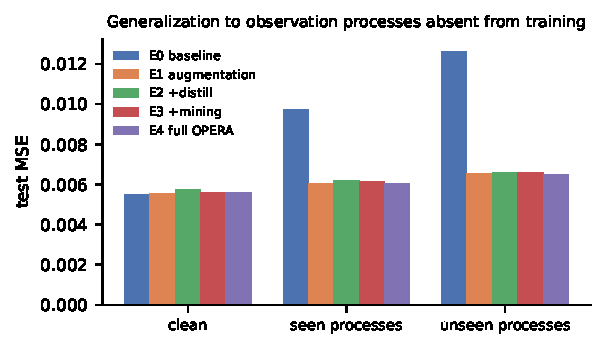
\includegraphics[width=0.85\linewidth]{figures/fig4_unseen_generalization.pdf}
\caption{Generalisation across the observation-process split on PhysioNet\prelim. ``Seen'' averages families
present in the training pool at unseen severities; ``unseen'' averages the nine conditions whose families never
appear in training (Section~\ref{sec:splits}). The gap between the two bars is small for every OPERA
configuration and large without any mechanism.}
\label{fig:unseen}
\end{figure}

\paragraph{Robustness extends to unseen process families.}
Figure~\ref{fig:unseen} separates conditions whose families appear in the training pool from those whose do
not. Without a mechanism the unseen group is worse than the seen group ($0.01260$ vs.\ $0.00975$) and both are
far above clean; with augmentation the three bars are nearly level ($0.00553$, $0.00604$, $0.00652$). The
mechanism therefore generalises across the split defined in Section~\ref{sec:splits} rather than memorising the
training pool.

\paragraph{Across settings, benefit tracks baseline damage.}
Table~\ref{tab:main} compares no mechanism against the full framework on every setting. Where degradation is
large the gains are large; where the baseline is already insensitive there is little to recover, and the
framework neither helps nor harms materially. On the classification tasks the effect appears in the primary
metric: PAM recovers $10.5$ and $11.1$ accuracy points at 30\% and 50\% variable removal, P19 gains $5.6$ AUROC
at 30\% variable removal and improves clean accuracy as well, and P12 --- which barely degrades --- gains $2.6$
AUROC at 50\% variable removal for a $0.2$ AUROC clean cost.

\begin{table}[t]
\caption{No mechanism vs.\ the full framework across all settings\prelim. Primary metric; MSE lower-better,
AUROC/accuracy higher-better. $\Delta$ is Eq.~\ref{eq:degradation} on the primary error.}
\label{tab:main}
\small
\begin{tabular}{llrrrr}
\toprule
 &  & \multicolumn{2}{c}{no mechanism} & \multicolumn{2}{c}{full OPERA} \\
\cmidrule(lr){3-4}\cmidrule(lr){5-6}
setting & metric & clean & $\Delta$ & clean & $\Delta$ \\
\midrule
Activity & MSE & \textbf{0.00263} & $+1793\%$ & 0.00286 & $\mathbf{+25\%}$ \\
PhysioNet & MSE & \textbf{0.00549} & $+107\%$ & 0.00559 & $\mathbf{+13\%}$ \\
PAM & acc. & \textbf{88.01} & $+64\%$ & 87.27 & $\mathbf{+34\%}$ \\
USHCN-12mo & MSE & 0.52020 & $+3.7\%$ & \textbf{0.51686} & $\mathbf{+2.6\%}$ \\
P19 & AUROC & 82.13 & $+2.9\%$ & \textbf{85.59} & $\mathbf{+1.2\%}$ \\
USHCN-1mo & MSE & 0.53787 & $+1.9\%$ & \textbf{0.52107} & $\mathbf{+1.5\%}$ \\
P12 & AUROC & \textbf{83.53} & --- & 83.30 & --- \\
\bottomrule
\end{tabular}
\end{table}

\begin{figure}[t]
\centering
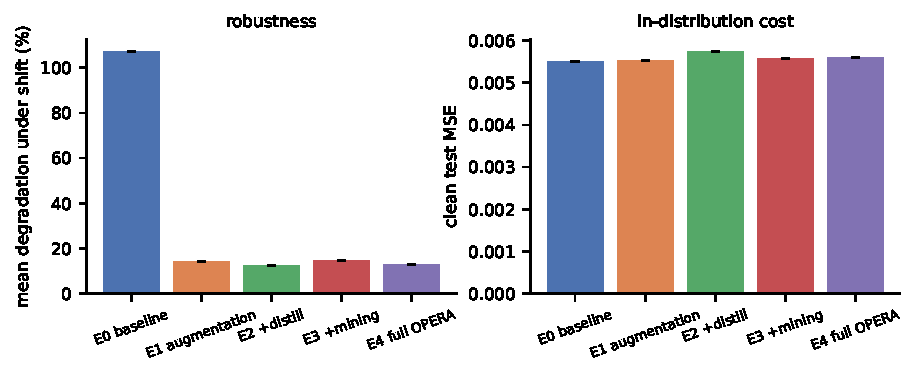
\includegraphics[width=\linewidth]{figures/fig5_ablation.pdf}
\caption{Contribution of each mechanism on PhysioNet\prelim: mean degradation under shift (left, lower is
better) against in-distribution error (right). Robustness improves by roughly an order of magnitude while
clean error moves within $0.0004$\,MSE, so the mechanisms are not trading in-distribution accuracy for
robustness.}
\label{fig:ablation}
\end{figure}

\paragraph{Cost.}
Figure~\ref{fig:ablation} summarises the trade and Table~\ref{tab:cost} the overhead. Every mechanism is
training-time only: parameter count is identical
across configurations and inference latency is unchanged at $0.63$\,ms per series. Augmentation costs
$1.7\times$ time and $1.7\times$ peak memory for two views; mining adds $K$ forward passes per step.

\begin{table}[t]
\caption{Training and deployment cost on PhysioNet\prelim. Inference and parameter count are unaffected by
every mechanism.}
\label{tab:cost}
\small
\begin{tabular}{lrrrr}
\toprule
configuration & params & s/epoch & peak GB & infer.\ ms \\
\midrule
no mechanism & 129{,}153 & 24.1 & 3.7 & 0.630 \\
augmentation & 129{,}153 & 41.4 & 6.3 & 0.670 \\
$+$ distillation & 129{,}153 & 45.3 & 6.3 & 0.630 \\
$+$ mining (harsher pool) & 129{,}153 & 82.3 & 6.3 & 0.634 \\
all three (harsher pool) & 129{,}153 & 86.3 & 6.3 & 0.629 \\
\bottomrule
\end{tabular}
\end{table}
